\documentclass[a4paper,11pt]{report}

\usepackage{amsmath,amssymb,amsthm}
\usepackage{fullpage}
\usepackage{graphicx}

\usepackage{bussproofs}
\usepackage{mathpartir}
\usepackage{prooftrees}
\usepackage{color}
\usepackage{rotating}



\usepackage{tikz}
\usetikzlibrary{automata,positioning}
\usetikzlibrary{fit}

\newcommand*\circled[1]{\tikz[baseline=(char.base)]{
    \node[shape=circle,draw,inner sep=2pt] (char) {#1};}}

\makeatletter
\pgfmathdeclarefunction{alpha}{1}{%
  \pgfmathint@{#1}%
  \edef\pgfmathresult{\pgffor@alpha{\pgfmathresult}}%
}

\newcommand*{\until}{U}
\newcommand*{\disj}{\ ,\ }
\newcommand*{\A}{\square}  % Always
\newcommand*{\D}{\diamondsuit} % eventually

\newcommand*{\Pq}{(\top,\bot)}
\newcommand*{\pQ}{(\bot,\top)}
\newcommand*{\PQ}{(\top,\top)}
\newcommand*{\pq}{(\bot,\bot)}


% tikz
\usepackage{tikz}
\usetikzlibrary{snakes}


\author{Sylvain Julmy}
\date{\today}

\setlength{\parindent}{0pt}
\setlength{\parskip}{2.5pt}

\newtheorem*{thm}{Theorem}

\begin{document}

\begin{center}
  \Large{
    Automata on Infinite Structure\\
    Fall 2018
  }
  
  \noindent\makebox[\linewidth]{\rule{\linewidth}{0.4pt}}
  Exercice Sheet 9

  \vspace*{1cm}

  Author : Sylvain Julmy
  \noindent\makebox[\linewidth]{\rule{\linewidth}{0.4pt}}

  \begin{flushleft}
    Professor : Ultes-Nitsche Ulrich
    
    Assistant : Stammet Christophe
  \end{flushleft}

  \noindent\makebox[\linewidth]{\rule{\textwidth}{1pt}}
\end{center}

\section*{Exercise 1}

\subsection*{1 : $(ab^*)^\omega$}

\[
  0 \in Q_a \wedge \forall x.(x \in Q_a \to \exists y.(y \in Q_a \wedge x < y))
\]

\subsection*{2 : $(aaa)^+(a+b)^\omega$}

\[
  0 \in Q_a \wedge
  0 + 1 \in Q_a \wedge
  0 + 1 + 1 \in Q_a \wedge
  \forall x.( 0 + 1 + 1 < x \to (x \in Q_a \vee x \in Q_b))
\]

\section*{Exercise 2}

\subsection*{1. }

\[
  \mathcal{L}_1 = ab(ab)^\omega = (ab)^\omega
\]

\subsection*{2. }

\[
  \mathcal{L}_2 = aabb (aabb)^\omega = (aabb)^\omega
\]

\subsection*{3. }

\[
  \mathcal{L}_3 = aabb (
  (aabb)^\omega +
  (aabb)^*(aaab)^\omega +
  (aabb)^*(aaab)^*a^\omega )
\]

\section*{Exercise 3}


\begin{center}
  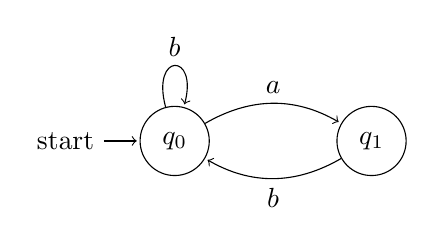
\begin{tikzpicture}[shorten >=1pt,node distance=2.5cm,on grid,auto]
    \tikzset{rounded/.style={draw,rectangle,rounded corners}}
    \node[state,initial] (q0) {$q_0$};
    \node[state] (q1) [right = of q0] {$q_1$};
    \path[->]
    (q0)
    edge [loop above] node [] {$b$} ()
    edge [bend left] node {$a$} (q1)
    (q1)
    edge [bend left] node {$b$} (q0)
    ;
  \end{tikzpicture}
\end{center}

  
\end{document}